\lab{Advanced Numpy}{Advanced Numpy}
\label{lab:NumPy}
\objective{NumPy is a vast library with many useful function that can be easily forgotten if not used and reviewed. This lab will help you remember some of its functionality that you may have forgotten and give you a few new functions to master.}

\begin{info}
Some of this lab is review, but there is new material near the end and additional materials beyond that.
\end{info}

\section*{Data Access} % ======================================================

\subsection*{Array Slicing} % -------------------------------------------------

Indexing for a 1-D NumPy array uses the slicing syntax \li{x[start:stop:step]}.
If there is no colon, a single entry of that dimension is accessed.
With a colon, a range of values is accessed.
For multi-dimensional arrays, use a comma to separate slicing syntax for each axis.

\begin{lstlisting}
# Make an array of the integers from 0 to 10 (exclusive).
>>> x = np.arange(10)
>>> x
array([0, 1, 2, 3, 4, 5, 6, 7, 8, 9])

# Access elements of the array with slicing syntax.
>>> x[3]                            # The element at index 3.
3
>>> x[:3]                           # Everything up to index 3 (exclusive).
array([0, 1, 2])
>>> x[3:]                           # Everything from index 3 on.
array([3, 4, 5, 6, 7, 8, 9])
>>> x[3:8]                          # The elements from index 3 to 8.
array([3, 4, 5, 6, 7])

>>> A = np.array([[0,1,2,3,4],[5,6,7,8,9]])
>>> A
array([[0, 1, 2, 3, 4],
       [5, 6, 7, 8, 9]])

# Use a comma to separate the dimensions for multi-dimensional arrays.
>>> A[1, 2]                         # The element at row 1, column 2.
7
>>> A[:, 2:]                        # All of the rows, from column 2 on.
array([[2, 3, 4],
       [7, 8, 9]])
\end{lstlisting}

% See Appendix \ref{appendix:numpy-visual-guide} for visual examples of slicing.

\begin{info} % Views vs. Copies.
Indexing and slicing operations return a \emph{view} of the array.
Changing a view of an array also changes the original array.
In other words, \textbf{arrays are mutable}.
To create a copy of an array, use \li{np.copy()} or the array's \li{copy()} method.
Changes to a copy of an array does not affect the original array, but copying an array uses more time and memory than getting a view.
\end{info}

\subsection*{Fancy Indexing} % ------------------------------------------------

So-called \emph{fancy indexing} is a second way to access or change the elements of an array.
Instead of using slicing syntax, provide either an array of indices or an array of boolean values (called a \emph{mask}) to extract specific elements.

\begin{lstlisting}
>>> x = np.arange(0, 50, 10)        # The integers from 0 to 50 by tens.
>>> x
array([ 0, 10, 20, 30, 40])

# An array of integers extracts the entries of 'x' at the given indices.
>>> index = np.array([3, 1, 4])     # Get the 3rd, 1st, and 4th elements.
>>> x[index]                        # Same as np.array([x[i] for i in index]).
array([30, 10, 40])

# A boolean array extracts the elements of 'x' at the same places as 'True'.
>>> mask = np.array([True, False, False, True, False])
>>> x[mask]                         # Get the 0th and 3rd entries.
array([ 0, 30])
\end{lstlisting}

Fancy indexing is especially useful for extracting or changing the values of an array that meet some sort of criterion.
Use comparison operators like \li{<} and \li{==} to create masks.

\begin{lstlisting}
>>> y = np.arange(10, 20, 2)        # Every other integers from 10 to 20.
>>> y
array([10, 12, 14, 16, 18])

# Extract the values of 'y' larger than 15.
>>> mask = y > 15                   # Same as np.array([i > 15 for i in y]).
>>> mask
<<array([False, False, False,  True,  True], dtype=bool)>>
>>> y[mask]                         # Same as y[y > 15]
array([16, 18])

# Change the values of 'y' that are larger than 15 to 100.
>>> y[mask] = 100
>>> print(y)
[10 12 14  100  100]
\end{lstlisting}

While indexing and slicing always return a view, fancy indexing always returns a copy.

\begin{problem} % Slicing / Fancy Indexing
Write a function that accepts a single array as input.
Make a copy of the array, then use fancy indexing to set all negative entries of the copy to $0$.
Return the resulting array.
\end{problem}

\section*{Array Manipulation} % ===============================================

\subsection*{Shaping} % -------------------------------------------------------

An array's \li{shape} attribute describes its dimensions.
Use \li{np.reshape()} or the array's \li{reshape()} method to give an array a new shape.
The total number of entries in the old array and the new array must be the same in order for the shaping to work correctly.
Using a \li{-1} in the new shape tuple makes the specified dimension as long as necessary.
% Whenever possible, \li{np.reshape()} returns a view.

\begin{lstlisting}
>>> A = np.arange(12)               # The integers from 0 to 12 (exclusive).
>>> print(A)
[ 0  1  2  3  4  5  6  7  8  9 10 11]

# 'A' has 12 entries, so it can be reshaped into a 3x4 matrix.
>>> A.reshape((3,4))                # The new shape is specified as a tuple.
array([[ 0,  1,  2,  3],
       [ 4,  5,  6,  7],
       [ 8,  9, 10, 11]])

# Reshape 'A' into an array with 2 rows and the appropriate number of columns.
>>> A.reshape((2,-1))
array([[ 0,  1,  2,  3,  4,  5],
       [ 6,  7,  8,  9, 10, 11]])
\end{lstlisting}

Use \li{np.ravel()} to flatten a multi-dimensional array into a 1-D array and \li{np.transpose()} or the \li{T} attribute to transpose a 2-D array in the matrix sense.

\begin{lstlisting}
>>> A = np.arange(12).reshape((3,4))
>>> A
array([[ 0,  1,  2,  3],
       [ 4,  5,  6,  7],
       [ 8,  9, 10, 11]])

# Flatten 'A' into a one-dimensional array.
>>> np.ravel(A)                     # Equivalent to A.reshape(A.size)
array([ 0,  1,  2,  3,  4,  5,  6,  7,  8,  9, 10, 11])

# Transpose the matrix 'A'.
>>> A.T                             # Equivalent to np.transpose(A).
array([[ 0,  4,  8],
       [ 1,  5,  9],
       [ 2,  6, 10],
       [ 3,  7, 11]])
\end{lstlisting}

\begin{info} % All 1-D Numpy arrays are flat!
By default, all NumPy arrays that can be represented by a single dimension, including column slices, are automatically reshaped into ``flat'' 1-D arrays.
For example, by default an array will have 10 elements instead of 10 arrays with one element each.
Though we usually represent vectors vertically in mathematical notation, NumPy methods such as \li{dot()} are implemented to purposefully work well with 1-D ``row arrays''.

\begin{lstlisting}
>>> A = np.arange(10).reshape((2,5))
>>> A
array([[0, 1, 2, 3, 4],
       [5, 6, 7, 8, 9]])

# Slicing out a column of A still produces a "flat" 1-D array.
>>> x = A[:,1]                      # All of the rows, column 1.
>>> x
array([1, 6])                       # Not array([[1],
>>> x.shape                         #            [6]])
(2,)
>>> x.ndim
1
\end{lstlisting}

However, it is occasionally necessary to change a 1-D array into a ``column array''.
Use \li{np.reshape()}, \li{np.vstack()}, or slice the array and put \li{np.newaxis} on the second axis.
Note that \li{np.transpose()} does not alter 1-D arrays.

\begin{lstlisting}
>>> x = np.arange(3)
>>> x
array([0, 1, 2])

>>> x.reshape((-1,1))               # Or x[:,np.newaxis] or np.vstack(x).
array([[0],
       [1],
       [2]])
\end{lstlisting}

Do not force a 1-D vector to be a column vector unless necessary.
\end{info}

\subsection*{Stacking} % ------------------------------------------------------

NumPy has functions for \emph{stacking} two or more arrays with similar dimensions into a single block matrix.
Each of these methods takes in a single tuple of arrays to be stacked in sequence.

\begin{table}[H]
\centering
\begin{tabular}{r|l}
    Function & Description\\
    \hline
    % % Shaping methods, already discussed
    % \li{reshape()} & Return a view of the array with a changed shape.\\
    % \li{ravel()} & Make a flattened version of an array, return a view if possible.\\
    % \li{transpose()} & Permute the dimensions of the array (also \li{ndarray.T}).\\
    % \hline
    \li{concatenate()} & Join a sequence of arrays along an existing axis\\
    \li{hstack()} & Stack arrays in sequence horizontally (column wise).\\
    \li{vstack()} & Stack arrays in sequence vertically (row wise).\\
    \li{column_stack()} & Stack 1-D arrays as columns into a 2-D array.
\end{tabular}
\end{table}

\begin{lstlisting}
>>> A = np.arange(6).reshape((2,3))
>>> B = np.zeros((4,3))

# vstack() stacks arrays vertically (row-wise).
>>> np.vstack((A,B,A))
array([[ 0.,  1.,  2.],             # A
       [ 3.,  4.,  5.],
       [ 0.,  0.,  0.],             # B
       [ 0.,  0.,  0.],
       [ 0.,  0.,  0.],
       [ 0.,  0.,  0.],
       [ 0.,  1.,  2.],             # A
       [ 3.,  4.,  5.]])

>>> A = A.T
>>> B = np.ones((3,4))

# hstack() stacks arrays horizontally (column-wise).
>>> np.hstack((A,B,A))
array([[ 0.,  3.,  1.,  1.,  1.,  1.,  0.,  3.],
       [ 1.,  4.,  1.,  1.,  1.,  1.,  1.,  4.],
       [ 2.,  5.,  1.,  1.,  1.,  1.,  2.,  5.]])

# column_stack() stacks arrays horizontally, including 1-D arrays.
>>> np.column_stack((A, np.zeros(3), np.ones(3), np.full(3, 2)))
array([[ 0.,  3.,  0.,  1.,  2.],
       [ 1.,  4.,  0.,  1.,  2.],
       [ 2.,  5.,  0.,  1.,  2.]])
\end{lstlisting}
%
See \url{http://docs.scipy.org/doc/numpy-1.10.1/reference/routines.array-manipulation.html} for more array manipulation routines and documentation.

\subsection*{Working with Dimensions}

In many scientific disciplines, arrays of more than 2 dimensions are readily utilized. Numpy's function are designed to work on these larger arrays but sometimes it's necessary to convert arrays to a different dimension. To do this we'll use \li{np.squeeze()} and \li{np.dstack}

\li{np.squeeze()} eliminates any superfluous dimensions in an array. These will be any dimension of value 1 when the shape attribute is called. It does not matter in which position the dimension is located. As a result of this, using \li{np.squeeze()} on several arrays of different shape can result in arrays of the same shape.

\begin{lstlisting}

# Define 3 arrays of different dimensions
>>> test0 = np.arange(9).reshape(1,3,3)
>>> test1 = np.arange(9).reshape(3,1,3)
>>> test2 = np.arange(9).reshape(3,3,1)

# but all arrays become the same after being squeezed
>>> np.squeeze(test0)
array([[ 0.,  1.,  2.],
       [ 3.,  4.,  5.],
       [ 6.,  7.,  8.]])

>>> np.squeeze(test1)
array([[ 0.,  1.,  2.],
       [ 3.,  4.,  5.],
       [ 6.,  7.,  8.]])

>>> np.squeeze(test2)
array([[ 0.,  1.,  2.],
       [ 3.,  4.,  5.],
       [ 6.,  7.,  8.]])

# even arrays with many extra dimensions reduce to the same matrix
>>> ridiculous = np.arange(9).reshape(1,1,1,1,3,3,1,1,1,1)
>>> np.squeeze(ridiculous)
array([[ 0.,  1.,  2.],
       [ 3.,  4.,  5.],
       [ 6.,  7.,  8.]])

# however arrays that have no 1 value in their shape will remain the same
>>> stoic = np.arange(20).reshape(2,2,5)
>>> print(stoic)
array([[[ 0,  1,  2,  3,  4],
        [ 5,  6,  7,  8,  9]],

       [[10, 11, 12, 13, 14],
        [15, 16, 17, 18, 19]]])

>>> print(np.squeeze(stoic))
array([[[ 0,  1,  2,  3,  4],
        [ 5,  6,  7,  8,  9]],

       [[10, 11, 12, 13, 14],
        [15, 16, 17, 18, 19]]])

\end{lstlisting} 

\li{np.dstack()}, on the other hand, performs like the other two stacking function except that it stacks on the third dimensions rather than the first or second. For example, using \li{np.dstack()} on two matrices of shape $(3,3)$ would make a matrix of shape $(3,3,2)$. If a matrix already has three dimensions or more, \li{np.dstack()} will only affect the third one (i.e, shapes $(3,3,2,2)$ with $(3,3,2,2)$ will create $(3,3,4,2)$)

\begin{problem}
Write a function that accepts a list of arrays, squeezes them and pads them with 0's so they are the same dimensions and then stacks them along the 3rd dimension. Thus, the arrays in the list can, individually, be any size and dimension. However, you may assume the arrays will all be 2-dimensional once the extra dimensions are squeezed out.

Hint: Use the various stacking commands to pad the inputted arrays appropriately with 0's so that they can easily be stacked into the three dimensional array in the end. Again, you may assume all arrays in the list, once squeezed, will be two dimensional arrays.
\end{problem}

\subsection*{Array Broadcasting} % --------------------------------------------

Many matrix operations make sense only when the two operands have the same shape, such as element-wise addition.
\emph{Array broadcasting} extends such operations to accept some (but not all) operands with different shapes, and occurs automatically whenever possible.

Suppose, for example, that we would like to add different values to the columns of an $m\times n$ matrix $A$.
Adding a 1-D array $x$ with the $n$ entries to $A$ will automatically do this correctly.
To add different values to the different rows of $A$, first reshape a 1-D array of $m$ values into a column array.
Broadcasting then correctly takes care of the operation.

Broadcasting can also occur between two 1-D arrays, once they are reshaped appropriately.

\begin{lstlisting}
>>> A = np.arange(12).reshape((4,3))
>>> x = np.arange(3)
>>> A
array([[ 0,  1,  2],
       [ 3,  4,  5],
       [ 6,  7,  8],
       [ 9, 10, 11]])
>>> x
array([0, 1, 2])

# Add the entries of 'x' to the corresponding columns of 'A'.
>>> A + x
array([[ 0,  2,  4],
       [ 3,  5,  7],
       [ 6,  8, 10],
       [ 9, 11, 13]])

>>> y = np.arange(0, 40, 10).reshape((4,1))
>>> y
array([[ 0],
       [10],
       [20],
       [30]])

# Add the entries of 'y' to the corresponding rows of 'A'.
>>> A + y
array([[ 0,  1,  2],
       [13, 14, 15],
       [26, 27, 28],
       [39, 40, 41]])

# Add 'x' and 'y' together with array broadcasting.
>>> x + y
array([[ 0,  1,  2],
       [10, 11, 12],
       [20, 21, 22],
       [30, 31, 32]])
\end{lstlisting}

\section*{Numerical Computing with NumPy} % ===================================

\subsection*{Universal Functions} % -------------------------------------------

A \emph{universal function} is one that operates on an entire array element-wise.
Universal functions are significantly more efficient than using a loop to operate individually on each element of an array.

\begin{table}[H]
\centering
\begin{tabular}{r|l}
    Function & Description \\
    \hline
    \li{<<abs()>>} or \li{absolute()} & Calculate the absolute value element-wise. \\
    % \li{conj()} & Return the complex conjugate of the array.\\
    \li{exp()} / \li{log()} & Exponential ($e^x$) / natural log element-wise.\\
    \li{maximum()} / \li{minimum()}& Element-wise maximum / minimum of two arrays.\\
    % \li{<<round()>>} & Return a rounded version of the array.\\
    \li{sqrt()} & The positive square-root, element-wise.\\
    \li{sin()}, \li{cos()}, \li{tan()}, etc. & Element-wise trigonometric operations.
\end{tabular}
\label{table:ufuncs}
\end{table}

\begin{lstlisting}
>>> x = np.arange(-2,3)
>>> print(x, np.<<abs>>(x))             # Like np.array([abs(i) for i in x]).
[-2 -1  0  1  2] [2 1 0 1 2]

>>> np.sin(x)                       # Like np.array([math.sin(i) for i in x]).
array([-0.90929743, -0.84147098,  0.        ,  0.84147098,  0.90929743])
\end{lstlisting}

\begin{problem}
Write a function that accepts a universal function and an $n\times n$ NumPy array, and returns how many times as fast it is to operate on the entire array element-wise, rather than by using a nested for loop to operate on each element individually. Run each way of operating on the matrix 10 times, and return the ratio of the averages of the two methods. Vow that you will avoid unnecessary nested for loops, especially when operating on large arrays.
\end{problem}

See \url{http://docs.scipy.org/doc/numpy/reference/ufuncs.html#available-ufuncs} for a more comprehensive list of universal functions.

\begin{warn}
The \li{math} module has many useful functions for numerical computations.
However, most of these functions can only act on single numbers, not on arrays.
NumPy functions can act on either scalars or entire arrays, but \li{math} functions tend to be a little faster for acting on scalars.
\begin{lstlisting}
>>> import math

# Math and NumPy functions can both operate on scalars.
>>> print(math.exp(3), np.exp(3))
20.085536923187668 20.0855369232

# However, math functions cannot operate on arrays.
>>> x = np.arange(-2, 3)
>>> np.tan(x)
array([ 2.18503986, -1.55740772,  0.        ,  1.55740772, -2.18503986])
>>> math.tan(x)
<<Traceback (most recent call last):
  File "<stdin>", line 1, in <module>
TypeError: only length-1 arrays can be converted to Python scalars>>
\end{lstlisting}
Always use universal NumPy functions, not the \li{math} module, when working with arrays.
\end{warn}

\subsection*{Other Array Methods} % -------------------------------------------

The \li{np.ndarray} class itself has many useful methods for numerical computations.

\begin{table}[H]
\centering
\begin{tabular}{r|l}
    Method & Returns \\
    \hline
    \li{<<all()>>} & \li{True} if all elements evaluate to \li{True}.\\
    \li{<<any()>>} & \li{True} if any elements evaluate to \li{True}.\\
    \li{argmax()} & Index of the maximum value.\\
    \li{argmin()} & Index of the minimum value.\\
    \li{argsort()} & Indices that would sort the array.\\
    \li{clip()} & restrict values in an array to fit within a given range\\
    \li{<<max()>>} & The maximum element of the array.\\
    \li{mean()} & The average value of the array.\\
    \li{<<min()>>} & The minimum element of the array.\\
    \li{roll()} & shuffles the elements of the array according to specified amount.\\
    \li{sort()} & Return nothing; sort the array in-place.\\
    \li{std()} & The standard deviation of the array.\\
    \li{<<sum()>>} & The sum of the elements of the array.\\
    % \li{trace()} & return the sum of the elements along the main diagonal\\
    \li{var()} & The variance of the array.\\
\end{tabular}
\label{table:ndarraymethods}
\end{table}

Each of these \li{np.ndarray} methods has an equivalent NumPy function.
For example, \li{A.<<max>>()} and \li{np.<<max>>(A)} operate the same way.
The one exception is the \li{sort()} function: \li{np.sort()} returns a sorted copy of the array, while \li{A.sort()} sorts the array in-place and returns nothing.

Every method listed can operate \emph{along an axis} via the keyword argument \li{axis}.
If \li{axis} is specified for a method on an $n$-D array, the return value is an $(n-1)$-D array, the specified axis having been collapsed in the evaluation process.
If \li{axis} is not specified, the return value is usually a scalar.
Refer to the NumPy Visual Guide in the appendix for more visual examples.

\begin{lstlisting}
>>> A = np.arange(9).reshape((3,3))
>>> A
array([[0, 1, 2],
       [3, 4, 5],
       [6, 7, 8]])

# Find the maximum value in the entire array.
>>> A.<<max>>()
8

# Find the minimum value of each column.
>>> A.<<min>>(axis=0)                   # np.array([min(A[:,i]) for i in range(3)])
array([0, 1, 2])

# Compute the sum of each row.
>>> A.<<sum>>(axis=1)                   # np.array([sum(A[i,:]) for i in range(3)])
array([3, 12, 21])
\end{lstlisting}

See \url{http://docs.scipy.org/doc/numpy/reference/generated/numpy.ndarray.
html} for a more comprehensive list of array methods.

\begin{problem} % Row stochastic matrices.
A matrix is called \emph{row-stochastic}\footnote{Similarly, a matrix is called \emph{column-stochastic} if its columns each sum to $1$.} if its rows each sum to $1$.
Stochastic matrices are fundamentally important for finite discrete random processes and some machine learning algorithms.

Write a function than accepts a matrix (as a 2-D NumPy array).
Divide each row of the matrix by the row sum and return the new row-stochastic matrix.
Use array broadcasting and the \li{axis} argument instead of a loop.
\end{problem}

\subsection*{Vectorizing functions}

Whenever possible making your functions `numpy aware' can greatly reduce complexity, increase readability and simplicity of code and make functions more versatile. Designing functions to be able to work with and utilize numpy arrays and numpy functions is one of the best ways to optimize code. However, sometimes the functions we need to use are very difficult to vectorize. In this case it can be useful to employ \li{np.vectorize()}

\li{np.vectorize()} accepts as an argument a function whose input and output is a scalar. It returns a new function that is `numpy aware', meaning that it will accept a numpy array of values and output an array where each entry had the operation defined by the original function performed on it.

\begin{lstlisting}
# Define a function to double a number
>>> def Double(x):           
...		return 2*x

>>> test = np.array([1,2,3,4,5])
# Using a for loop we can get the doubled array
>>> for i,val in enumerate(test):   
...		test[i] *= 2
>>> test
array([2,4,6,8,10])

# Vectorizing our Double function
>>> DoubleVectorized = np.vectorize(Double)   

>>> test = np.array([1,2,3,4,5])
# with the function vectorized the implementation is simple
>>> DoubleVectorized(test)     
array([2,4,6,8,10])

\end{lstlisting}

\begin{info} %warning that this function does not actually help with complexity

While the above example can easily be done with array broadcasting, \li{np.vectorize()} can be implemented with very complex scalar functions for which no array broadcasting method exists. However, it should be noted that this function is used only for convenience and readability since it does not improve temporal complexity like normal array broadcasting would. Even though it doesn't improve the complexity, it is often simpler than trying to formulate the for loop.

\end{info}

\begin{problem}

Given to you is the code that finds the prime factorization of a number and returns the largest prime in the factorization. Vectorize the function using \li{np.vectorize()} and program a function that either uses the vectorized function or the naive for loop depending on the argument `naive' being passed in as True or False. 

Make sure you function returns a numpy array of the same size for both cases.

\noindent Hint: Make sure the naive approach returns the array with a dtype of `int32'

\end{problem}

\section*{Einsum}

While numpy has many functions to help multiply arrays, multiplying the elements of arrays in unorthodox ways usually requires the conglomeration of quite a few of these functions. \li{np.einsum()} is designed to eliminate this problem by making a general framework for multiplication and addition in arrays using their shapes and allowing the coder to tell the function which elements exactly are to be multiplied or summed and how those operations are to be returned.

The \li{np.einsum()} function can be used on arrays of greater than 2 dimensions, but we'll keep the scope of this text to working with input arrays of 1 or 2 dimensions. The numbers in the following syntax only represent positions, each position will be explained below:

\begin{center}
\li{np.einsum("12,34 -> 56", 7, 8)}
\end{center}

The meaning of the positions are as follows:

\begin{enumerate}
\item[\textcolor{magenta}{1} and \textcolor{magenta}{2})] The variables representing the shape of the first input array (the variables will be explained later). In the case of 1 dimensional vectors, there will only be one variable and the second will be omitted.
\item[\textcolor{magenta}{3} and \textcolor{magenta}{4})] Similarly, the variables representing the shape of the second input array.
\item[\textcolor{magenta}{5} and \textcolor{magenta}{6})] The variables representing the dimensions of the output array. There can one, two, or even three variables here.
\item[\textcolor{white}{easter} \textcolor{magenta}{7})] The first input array. Make sure it is outside the quotation mark ending the variables section and preceded by a comma.
\item[\textcolor{white}{e g g!} \textcolor{magenta}{8})] The second input array.
\end{enumerate}

Positions 7 and 8 are obviously arrays, but position 1-6 are filled with the variables, usually $i$, $j$, and $k$ which represent the dimensions of the input and output arrays. Einsum can multiply and/or sum any two matrices across any axis by simply changing the way these variables are arranged and repeated.

\subsection*{Einsum Rules}

The way \li{einsum()} interprets its inputted variables are as follows:

\begin{enumerate}
\item[1)] If the variables contained in positions 1 or 2 share a variable in 3 or 4, the values along the axes specified by the repeated variables positions will be multiplied together.\\

\item[2)] On the other side of the arrow (positions 5 and 6), specify the dimensions of the output. Ommiting a variable from these positions causes the products to be summed.
\end{enumerate}

\noindent As an example, we will define normal matrix multiplication using einsum.

\begin{lstlisting}
>>> import numpy as np

>>> A = np.eye(3)
>>> A[0,:] += A[2,:]
>>> A
array([[1, 0, 1],
       [0, 1, 0],
       [0, 0, 1]])

>>> B = np.arange(9).reshape((3,3))
>>> B
array([[0, 1, 2],
       [3, 4, 5],
       [6, 7, 8]])

# We use einsum to define normal matrix multiplication
# note the 'j' is repeated in axis 1 and axis 0 respectively
>>> np.einsum("ij,jk -> ik", A, B) 
array([[6, 8, 10],
       [3, 4, 5],
       [6, 7, 8]])

\end{lstlisting}

Since the \li{j} was repeated in the previous example, the elements on those 2 axes are paired and multiplied. The first pair of indicies has \li{j} in the second position, which corresponds to the column position (axis=1; moving from column to column down a single row). The second pair of indices has \li{j} in the first position, which corresponds to the row position (axis=0; moving row to row down a single column). Thus, Einsum takes products of the elements along the respective column and row pairs in exactly the same way as matrix multiplication.
The output was specified to be \li{ik} instead of \li{ijk}, so einsum summed the products that it created from having the repeated \li{j}.
It's important to note here that Einsum adds and multiplies in a very similar manner to the \li{axis} argument in \li{np.sum()} and other numpy functions.

\subsection*{Other operations from einsum}

\begin{enumerate}
\item[\textbf{Transpose:}] If only one matrix is inputted (position 8 is ommited) then several operations can be done by rearranging the input variables. The transpose is accomplished by switching the axes variables: \li{np.einsum("ij -> ji", A)}
\item[\textbf{Row sums:}] Here the variable representing the row axis must be ommitted so einsum sums the rows (note no products were taken but the summing is still allowed. \li{np.einsum("ij -> j", A)}
\item[\textbf{Column sums:}] Summing the columns is similar \li{np.einsum("ij -> i", A)}
\item[\textbf{Dot product:}] Whenever your output is a scalar the arrow in the function is optional.\\ \li{np.einsum("i, i", x, y)} is equivalent to \li{np.einsum("i, i ->", x, y)}. Note here that the \li{i} must be repeated to get the proper dot product
\item[\textbf{Full matrix sum:}] Summing the entire matrix is similar to the dot product. \li{np.einsum("ij->",A)} 
 
\end{enumerate}

\begin{info}
While excluding a variables after the \li{->} symbol will cause summation along the corresponding axis to occur,  including the variables when usual matrix multiplication would exclude them can cause array broadcasting to occur on the input vectors or matrices. One of the next examples shows this.
\end{info}

Now, to demonstrate Einsum's true power we'll show a more complicated example. Imagine you needed to take an outer product of each column of a matrix with the corresponding column of another matrix. You could accomplish this in a for loop, but it would be slow and not very effective. Conversely, this can be done in one line with \li{np.einsum}.

\begin{lstlisting}
>>> A = np.arange(9).reshape((3,3))
>>> outer_products = np.einsum("ic, jc -> cij", A, A)
>>> outer_products
array([[[ 0,  0,  0],
        [ 0,  9, 18],
        [ 0, 18, 36]],

       [[ 1,  4,  7],
        [ 4, 16, 28],
        [ 7, 28, 49]],

       [[ 4, 10, 16],
        [10, 25, 40],
        [16, 40, 64]]])
\end{lstlisting} 

The output dimension having three variables creates a 3-dimensional matrix where each element in the first axis is a 3 by 3 outer product matrix. If we then wanted to sum the rows of each of those matrices and make a 2 dimensional matrix from these row sums, we simply omit the row axis variable \li{i}.

\begin{lstlisting}
>>> A = np.arange(9).reshape((3,3))
>>> outer_products_sum = np.einsum("ic, jc -> cj", A, A)
>>> outer_products_sum
array([[  0,  27,  54],
       [ 12,  48,  84],
       [ 30,  75, 120]])
\end{lstlisting}

And then perhaps we want to array broadcast a different vector to the rows of the resulting matrix. We can think of starting with our output variables \li{cj} and design it from there, adding to the already existing Einsum function. The vector variable needs to match the axis we want to iterate over. Since we want the elements of our vector to be distributed to the rows of the matrix, we choose \li{j} to represent our vector.

\begin{lstlisting}
>>> A = np.arange(9).reshape((3,3))
>>> v = np.array([0,1,-1])
>>> outer_product_sum_with_broadcast = np.einsum("ic, jc, j -> cj", A, A, v)
>>> outer_product_sum_with_broadcast
array([[   0,   27,  -54],
       [   0,   48,  -84],
       [   0,   75, -120]])
\end{lstlisting}

\noindent And thus, three difficult operations have been reduced to a few letters by the power of Einsum.

\subsection*{Einsum Optimize}

\li{np.einsum()}, in most cases, performs faster than built in numpy functions. However, the way Einsum organizes its operations creates redundancy when trying to perfrom multiple operations at once, such as multiplying two matrices, broadcasting a vector to its rows and then summing the resulting matrix columns. One should be cautious when using Einsum to perform multiple operations since you may actually be making your complexity worse rather than improving it. 

There are two ways around this problem. First, performing each operation individually will preserve the integrity of Einsum's performance, although brevity of code will suffer. Second, multiple operations can be performed efficiently using kwarg \li{optimize=True}.

Setting \li{optimize=True} creates an extra step of operational analysis before any calculations are made to ensure efficient order of operations. In addition, this mode uses a more spatially complex method of computation in exchange for ensured temporal gains. This is why \li{optimize} defaults to \li{False}: to allow the programmer to know whether or not there is sufficient memory or need for the optimize functionality.

\begin{problem}
Write a function that accepts 3 vectors and a matrix of appropriate sizes and returns a matrix that is the result of an outer product of the first 2 vectors, the 3rd vector array broadcasted to the columns of that matrix and then the multiplication via normal matrix multiplication of that result to the inputed matrix.

Hint: Your result should return the equivalent of \li{np.outer(x,y)*z.reshape(-1,1)@A} where x, y, and z are vectors and A is a matrix.
\label{prob:outer product}
\end{problem}

\begin{problem}
Time your einsum function from Problem \ref{prob:outer product} versus its numpy function equivalent for vectors of size 3 through 500 and arrays of size (3,3) through (500,500). Plot the results on a neatly formatted and labeled graph.

\noindent Hint: If your Einsum function is running slower than its numpy equivalent, consider using one of the two methods described above. In the end, your graphs should look like one of these:

\begin{figure}[H]
    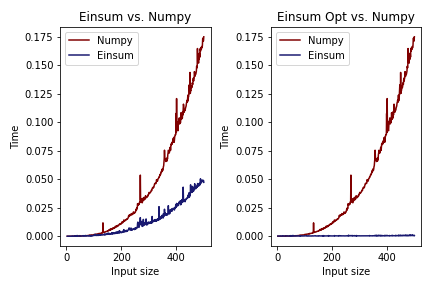
\includegraphics[width=.7\textwidth]{figures/Einsum_timing_plots.png}
\end{figure}

\end{problem}

\newpage

\section*{Additional Material} % ==============================================

\subsection*{Random Sampling} % -----------------------------------------------

The submodule \li{np.random} holds many functions for creating arrays of random values chosen from probability distributions such as the uniform, normal, and multinomial distributions.
It also contains some utility functions for getting non-distributional random samples, such as random integers or random samples from a given array.

\begin{table}[H] % The np.random submodule.
\begin{tabular}{r|l}
Function & Description\\
\hline
\li{choice()} & Take random samples from a 1-D array.\\
\li{random()} & Uniformly distributed floats over [0, 1).\\
\li{randint()} & Random integers over a half-open interval.\\
\li{random_integers()} & Random integers over a closed interval.\\
\li{randn()} & Sample from the standard normal distribution.\\
\li{permutation()} & Randomly permute a sequence / generate a random sequence.\\
\\
Function & Distribution\\
\hline
\li{beta()} & Beta distribution over [0, 1].\\
\li{binomial()} & Binomial distribution.\\
\li{exponential()} & Exponential distribution.\\
\li{gamma()} & Gamma distribution.\\
\li{geometric()} & Geometric distribution.\\
\li{multinomial()} & Multivariate generalization of the binomial distribution.\\
\li{multivariate_normal()} & Multivariate generalization of the normal distribution.\\
\li{normal()} & Normal / Gaussian distribution.\\
\li{poisson()} & Poisson distribution.\\
\li{uniform()} & Uniform distribution.
\end{tabular}
\end{table}

Note that many of these functions have counterparts in the standard library's \li{random} module.
These NumPy functions, however, are much better suited for working with large collections of random samples.

\begin{lstlisting}
# 5 uniformly distributed values in the interval [0, 1).
>>> np.random.random(5)
array([ 0.21845499,  0.73352537,  0.28064456,  0.66878454,  0.44138609])

# A 2x5 matrix (2-D array) of integers in the interval [10, 20).
>>> np.random.randint(10, 20, (2,5))
array([[17, 12, 13, 13, 18],
       [16, 10, 12, 18, 12]])
\end{lstlisting}

\subsection*{Saving and Loading Arrays} % -------------------------------------

It is often useful to save an array as a file for later use.
NumPy provides several easy methods for saving and loading array data.

\begin{table}[H]
\begin{tabular}{r|l}
Function & Description\\
\hline
\li{save()} & Save a single array to a \texttt{.npy} file.\\
\li{savez()} & Save multiple arrays to a \texttt{.npz} file.\\
\li{savetxt()} & Save a single array to a \texttt{.txt} file.\\
\hline
\li{load()} & Load and return an array or arrays from a \texttt{.npy} or \texttt{.npz} file.\\
\li{loadtxt()} & Load and return an array from a text file.
\end{tabular}
\end{table}

\begin{lstlisting}
# Save a 100x100 matrix of uniformly distributed random values.
>>> x = np.random.random((100,100))
>>> np.save("uniform.npy", x)       # Or np.savetxt("uniform.txt", x).

# Read the array from the file and check that it matches the original.
>>> y = np.load("uniform.npy")      # Or np.loadtxt("uniform.txt").
>>> np.allclose(x, y)               # Check that x and y are close entry-wise.
<<True>>
\end{lstlisting}

To save several arrays to a single file, specify a keyword argument for each array in \li{np.savez()}.
Then \li{np.load()} will return a dictionary-like object with the keyword parameter names from the save command as the keys.

\begin{lstlisting}
# Save two 100x100 matrices of normally distributed random values.
>>> x = np.random.randn(100,100)
>>> y = np.random.randn(100,100)
>>> np.savez("normal.npz", first=x, second=y)

# Read the arrays from the file and check that they match the original.
>>> arrays = np.load("normal.npz")
>>> np.allclose(x, arrays["first"])
<<True>>
>>> np.allclose(y, arrays["second"])
<<True>>
\end{lstlisting}

\begin{comment}
\subsection*{Polynomials} % ---------------------------------------------------

The \li{np.poly1d} object represents a polynomial in NumPy.
The constructor is called with the coefficients of the desired polynomial.

\begin{lstlisting}
>>> poly = np.poly1d([3, 5, 1, 2, 0, 1])
>>> print(poly)
   5     4     3     2
3 x + 5 x + 1 x + 2 x + 1
\end{lstlisting}

The object \li{poly} represents the polynomial $3x^5+5x^4+x^3+2x^2+1$.
NumPy provides many functions to operate on \li{poly1d} objects (see \url{http://docs.scipy.org/doc/numpy/reference/routines.polynomials.polynomial.html}).

Recall that
\[
e^x = \sum_{n=0}^{\infty} \frac{x^n}{n!}.
\]
The following function evaluates the $N$th partial sum of this series at the value $a$.

\begin{lstlisting}
>>> from scipy.special import factorial
>>> def exp(a, N=25):
...     """Construct an array in reverse order from n to 0."""
...     n = np.arange(N, -1, -1)
...     # Use broadcasting to compute coefficients
...     coeffs = 1. / factorial(n)
...     poly = np.poly1d(coeffs)        # Make a polynomial object.
...     return poly(a)
...
\end{lstlisting}

The last two lines can be condensed by using the following command:

\begin{lstlisting}
np.polyval(p, a)
\end{lstlisting}

\begin{problem}
\leavevmode
\begin{enumerate}
\item Use NumPy's polynomial objects to approximate the following series.
\[
\arcsin x = \sum_{n=0}^{\infty} \frac{\left(2 n\right) ! x^{2 n + 1}}{\left(2 n + 1\right)\left(n!\right)^2 4^n}
\]
This series converges on $(-1, 1)$. Use your series approximation to approximate $\pi$. Hint: think of the powers of $x$ that
are not included in the series as having zero coefficients.

\item The lambert W function is the inverse of $x e^x$.
Its Taylor series is below (note the index starts at 1).
\[
W(x) = \sum_{n=1}^{\infty} \frac{\left(-n\right)^{n-1} x^n}{n!}
\]
This series has a radius of convergence of $\frac{1}{e}$.
Use the series to approximate a number $x$ such that $x e^x = \frac{1}{4}$.
Verify that your approximation is close.
\end{enumerate}
\end{problem}
\end{comment}

\begin{comment}
\subsection*{Iterating Through Arrays} % --------------------------------------

Iterating through an array (using a \li{for} loop) negates most of the advantages of using NumPy.
Avoid iterating through arrays as much as possible by using array broadcasting and universal functions.
When absolutely necessary, use \li{np.nditer()} to create an efficient iterator for the array.
See \url{http://docs.scipy.org/doc/numpy/reference/arrays.nditer.html} for details.
\end{comment}